\chapter{Grammar of Graphics Tools}
The Grammar of Graphics by Leland Wilkinson is a framework that provides a unique foundation for producing almost every quantitative graphic found in scientific journals, newspapers, statistical packages, and data visualization systems.

\section*{The Layers: An Overview}
\begin{minipage}[t]{0.6\textwidth}
    \vspace{0pt}
    The Grammar of Graphics follows a layered approach to describe and construct visualizations or graphics. 
    It provides a common language for thinking about the ways that design choices are made in visualization, describing everything from the data used to the visual channels displayed on the marks, and how data is converted into those channels.
    \hspace{1cm}
\end{minipage}
\begin{minipage}[t]{0.4\textwidth}
    \vspace{0pt}
    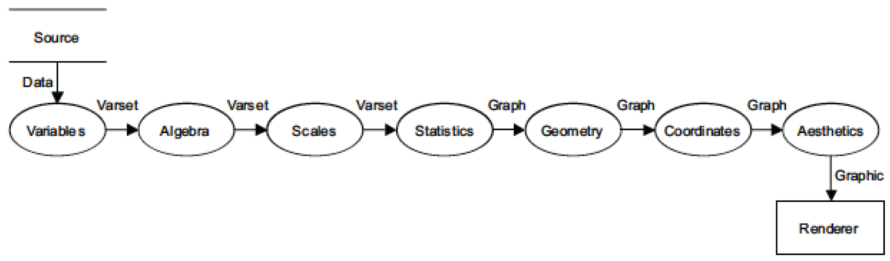
\includegraphics[width=\textwidth]{figures/grammar_flow.png}
    \captionof{figure}{Grammar of Graphics Flow \cite{wilkinsonHowMakePie2005}}
\end{minipage}
\captionsetup{justification=centering}

\vspace{-3mm}

\subsection*{Data}
\vspace{-2mm}
\begin{minipage}[t]{0.7\textwidth}
    In the first step, as described above, we aggregate the data we want to visualize. At this step, the visualization only consists of its bare minimum.
    \hspace{1cm}
\end{minipage}
\begin{minipage}[t]{0.3\textwidth}
    \vspace{-20pt}
    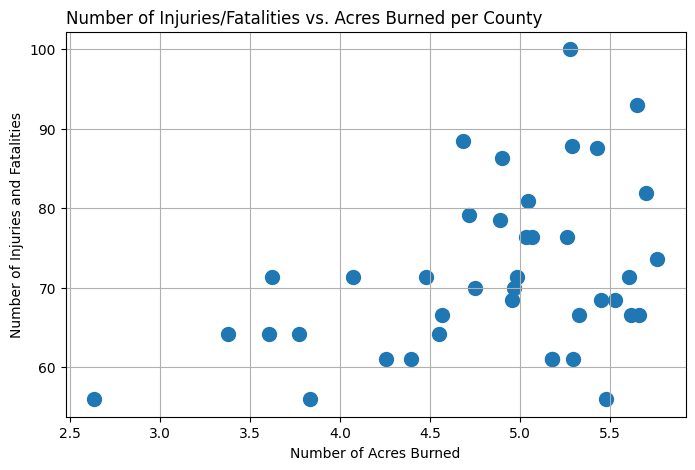
\includegraphics[width=\textwidth]{figures/gog_data.png}
    \captionof{figure}{Grammar of Graphics: Data}
\end{minipage}


\vspace{-3mm}

\subsection*{Aesthetics}
\vspace{-2mm}
\begin{minipage}[t]{0.6\textwidth}
    In the Grammar of Graphics, the Aestehetics Layer refers to the mapping of one or more variables to one or more visual elements on the graph. This includes 
    mapping variables to the x-axis, y-axis, and using color to differentiate different attributes. Aesthetics are essential in creating meaningful and 
    effective visualizations \cite{wilkinsonAesthetics2005}.
    In this example we map the \texttt{AcresBurned} variable to the x-axis and the sum of \texttt{Injuries} and \texttt{Fatalities} variables to the y-axis. Additionally,
    the Admin Units (fire departments) get added as a third dimension by using color.
    \hspace{1cm}
\end{minipage}
\begin{minipage}[t]{0.4\textwidth}
    \vspace{-20pt}
    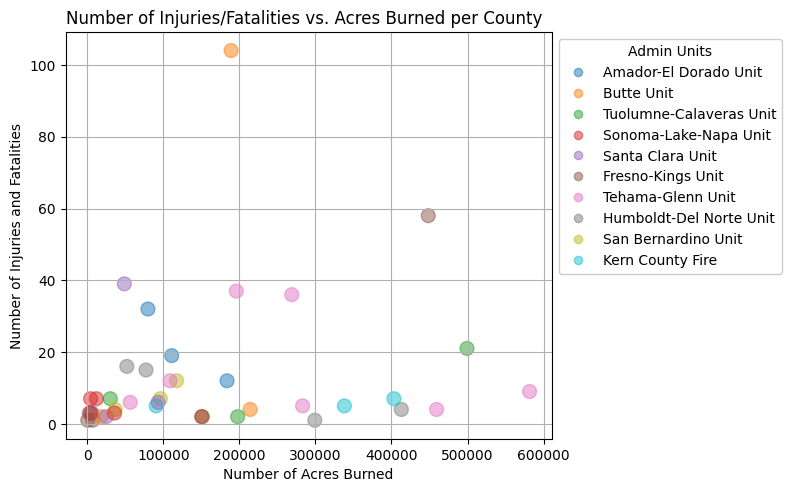
\includegraphics[width=\textwidth]{figures/gog_aesthetics.png}
    \captionof{figure}{Grammar of Graphics: Aesthetics}
\end{minipage}

\vspace{-3mm}

\subsection*{Scale}
\vspace{-2mm}
\begin{minipage}[t]{0.6\textwidth}
    In the Grammar of Graphics, the Scale step can include the scaling of the data, but 
    also the scaling of the visual elements, such as the axes or scatter sizes \cite{wilkinsonScales2005}.
    \hspace{1cm}
\end{minipage}%
\begin{minipage}[t]{0.4\textwidth}
    \vspace{-20pt}
    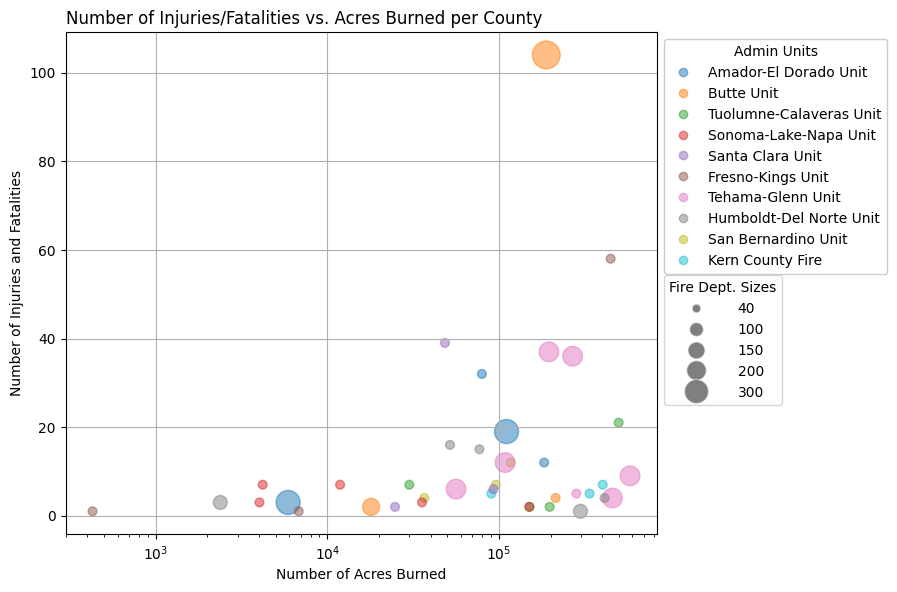
\includegraphics[width=\textwidth]{figures/gog_scale.png}
    \captionof{figure}{Grammar of Graphics: Scale}
\end{minipage}

\vspace{-2mm}

\subsection*{Geometry}
\vspace{-2mm}
\begin{minipage}[t]{0.6\textwidth}
    In the Grammar of Graphics
    \hspace{1cm}
\end{minipage}%
\begin{minipage}[t]{0.4\textwidth}
    \vspace{-20pt}
    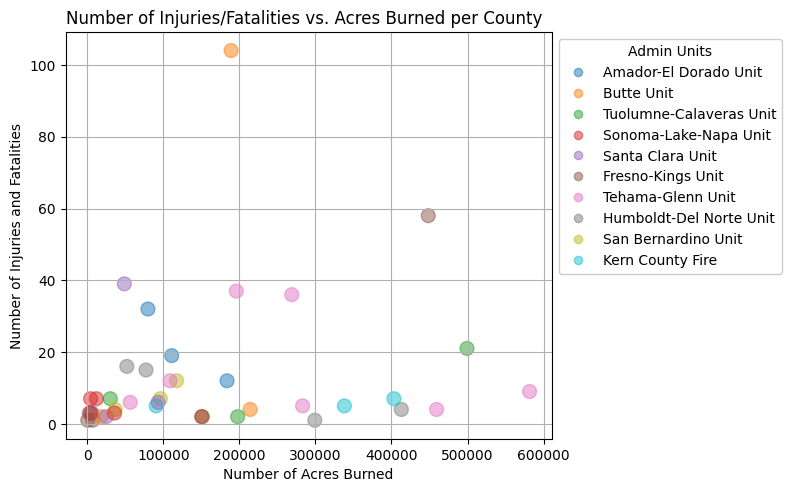
\includegraphics[width=\textwidth]{figures/gog_aesthetics.png}
    \captionof{figure}{Grammar of Graphics: Aesthetics}
\end{minipage}

\vspace{-2mm}

\subsection*{Statistics}
\vspace{-2mm}
\begin{minipage}[t]{0.6\textwidth}
    In the Grammar of Graphics
    \hspace{1cm}
\end{minipage}%
\begin{minipage}[t]{0.4\textwidth}
    \vspace{-20pt}
    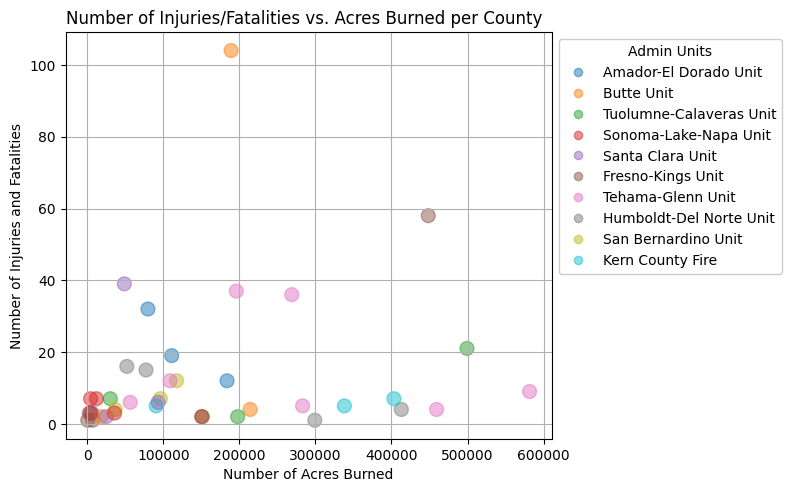
\includegraphics[width=\textwidth]{figures/gog_aesthetics.png}
    \captionof{figure}{Grammar of Graphics: Aesthetics}
\end{minipage}

\vspace{-2mm}

\subsection*{Facets}
\vspace{-2mm}
\begin{minipage}[t]{0.6\textwidth}
    In the Grammar of Graphics
    \hspace{1cm}
\end{minipage}%
\begin{minipage}[t]{0.4\textwidth}
    \vspace{-20pt}
    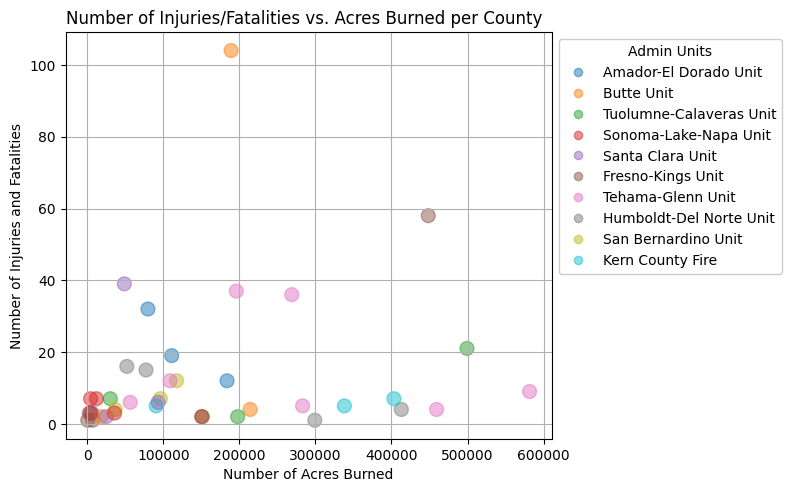
\includegraphics[width=\textwidth]{figures/gog_aesthetics.png}
    \captionof{figure}{Grammar of Graphics: Aesthetics}
\end{minipage}

\vspace{-2mm}

\subsection*{Coordinates}
\vspace{-2mm}
\begin{minipage}[t]{0.6\textwidth}
    In the Grammar of Graphics
    \hspace{1cm}
\end{minipage}%
\begin{minipage}[t]{0.4\textwidth}
    \vspace{-20pt}
    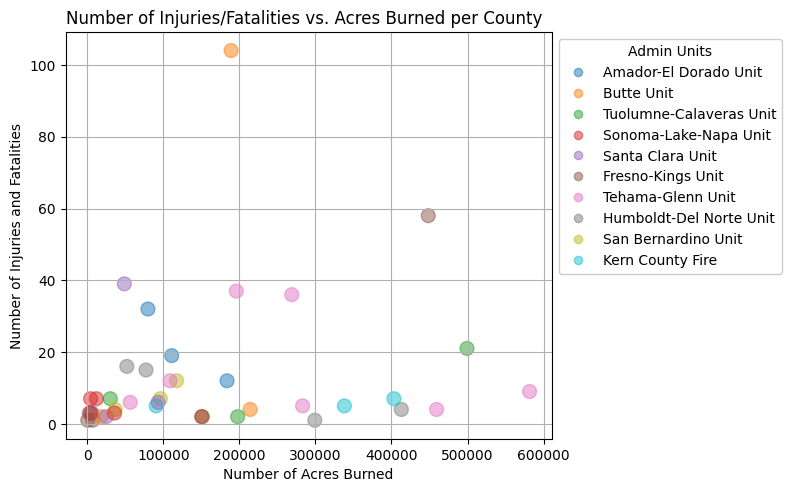
\includegraphics[width=\textwidth]{figures/gog_aesthetics.png}
    \captionof{figure}{Grammar of Graphics: Aesthetics}
\end{minipage}